\begin{comment}
2.3 Teil II: SW-Projektdokumentation
Hier folgen die Dokumente gemäss Software-Engineering-Vorgehen.
2.3.1 Überblick
Zweck und Inhalt dieses Kapitels
2.3.2 Vision
Verweis auf Teil I.
2.3.3 Anforderungsspezifikation
Enthält folgende mögliche Unterkapitel:
 Rahmenbedingungen (wenn nicht schon oben abgehandelt)
 Anwendungsfalldiagramm
 Hauptanwendungsfall
 Funktionale Anforderungen
 Nicht-Funktionale Anforderungen
 Weitere: Aktivitätsdiagramme, Fallbeispiele, Szenarien, Prototypen...
2.3.4 Analyse
Klassen-, bzw. Domainmodell.
2.3.5 Design (Entwurf)
Die Architektur soll eine objektorientierte Problemdomain umfassen. Eine allfällig eingesetzte Datenbank darf diese Problemdomain permanent speichern, nicht aber ersetzen.
Enthält folgende mögliche Unterkapitel:
 Klassenverantwortlichkeiten (Klassenname, Verantwortlichkeit, Wissen, Tun, Abhängigkeiten); CRC- Diagramme?
 Sequenzdiagramm / Kollaborationsdiagramm
2.3.6 Implementation (Entwicklung)
Objektkatalog: könnte mit einem Thesaurus verwaltet werden! Rest individuell.
2.3.7 Test
Enthält folgende mögliche Unterkapitel:
 Testverfahren automatisch (mit JUnit) und manuell (dokumentiert; z.B. GUI); durchnummeriert.
 Iterationen 1 ... X
2.3.8 Resultate
Resultate und Ergebnisse der Arbeit. Dieser Abschnitt richtet sich an den speziell für das entsprechende Fachgebiet interessierten Ingenieur. Er soll es ihm ermöglichen, die für die Problemlösung gemachten Überlegungen zu verstehen und nachzuvollziehen.
2.3.9 Weiterentwicklung
Möglichkeiten der Weiterentwicklung: Funktionen und mögliches weiteres Vorgehen. Weiterentwicklung scheint allgemein ein heikler Punkt zu sein in allen Projekten, besonders auch in SA/DA-Projekten:
In realen Projekten, im RUP-Prozess wird er kaum betont und auch für Sie und für die Auftraggeber scheint es ein Problem zu sein. Warum?
 Wenn man dort zuviel aufschreibt, dann könnte das als Manko aufgefasst werden; und Aufschreiben nimmt erst noch Zeit weg...
 Zudem ist aus Sicht Auftraggeber (ohne "Gegensteuer") eine zusätzliche Funktion besser bewertbar als der "Wert" eines robusten, sauberen Designs oder eines Refactorings (z.B. der Separierung der Objekt/Klassen-Zuständigkeiten).
Ein Test, wie "sauber" - namentlich: wie änderungsfreundlich - ein Design ist, zeigt sich beispielsweise in der Antwort auf folgende Frage: "Welche Interfaces muss man implementieren und/oder welche Komponenten/Klassen muss man erweitern (schlimmstenfalls anpassen), um eine weitere Funktionalität einzubauen? Z.B. ein weiterer Exportfilter?".
Daher gelten folgende Regelungen zur Weiterentwicklung (gilt auch für andere Projektarten):
 Weiterentwicklung ist obligatorisch und erscheint in zwei separaten Kapitel (ggf. Dokument): Im Technischen Bericht, Unterkapitel Resultate/Ausblick, und in der SW-Projektdokumentation.
 Weiterentwicklung im Technischen Bericht ist allgemein gehalten und daher weniger heikel. Wichtig ist die Aufzählung der hauptsächlichen weiteren möglichen funktionalen oder nicht-funktionalen Anforderungen.
 Weiterentwicklung in der SW-Projektdokumentation ist an Architekten / SW-Entwickler gerichtet wie jedes andere SW-Dokument.
 Gewichtung: Es wird separat bewertet und zusätzlich erst spät (SA/DA bei der Präsentation) vollständig abgegeben wird. Spät heisst bei DAs auf der Dokumentation der Präsentation (inkl. CD). Sein ungewichtetes Gewicht gegenüber der Gesamtdokumentation ist umfangmässig ca. 1/15. Zur Erinnerung siehe Unterkapitel Lieferdokumente mit ca. 15 Hauptkapitel-/-Dokumenten.
2.3.10 Benutzerdokumentation
Installationsanleitung(en), Bedienungsanleitung(en) und Tutorien (evtl. in den Anhang)! Vergessen Sie a) nicht den CD-Inhalt zu notieren und auch in die Doku. zu nehmen.
Testen sie die Installation mit realistischen Vorgaben!!
2.4.1 Allgemeines
 Normen
 Konfigurationsmanagement (Entwicklungs-Werkzeuge, Eingesetzte Software)
2.4.2 Projektmanagement
Enthält folgende mögliche Unterkapitel:
 Vorgehen
 Zeitplanung
 (Erreichen der Ziele siehe sep. Kapitel "Bewertung und Ausblick").
Zeitplanung: Die Zeitplanung orientiert sich an den Meilensteinen und ist nach folgender Idee strukturiert:
     Inception => Elaboration => Construction 1 => Construction 2 => ... => Transition
Das ergibt folgendes Zeitdiagramm:
2.4.3
                          Dokumente
Dokumente Teil I:             |
+ Einführung                  |
+ Vision                      |
+ "Stand der Technik"         |
+ Umsetzungskonzept           |
+ Resultate                   |
Dokumente Teil II:            |
+ Anforderungsspezifikation   |
+ Analyse                     |
+ Design                      |
+ Implementation              |
+ Projektmgmt.&-Monitoring    |
+ Test                        |
+ Resultate und Weiterentw.   |
+ Benutzerdokumentation       |
+ Glossar und Abkürzungsverz. |
+ Literatur- und Quellenverz. |
                              +----+------+---------+---------+------> Tage
               Zeitabschnitte: Inc.  Elab.  Constr.1  Constr.2  Trans.
Projektmonitoring
Code-Analyse (Metriken).
\end{comment}

\part{Projektdokumentation}

\subimport{}{anforderungen.tex}

\chapter{Analyse}


\section{Datenspeicherung}
Ein Ziel dieser Arbeit ist die Erstellung eines Daten-Hubs, welcher es Anbietern ermöglicht, ihre Daten anderen zur Verfügung zu stellen. 

Zur Speicherung der Daten stehen folgende Varianten zur Auswahl.

\subsection{File-basiert}
Die Daten werden direkt im Dateisystem gespeichert. Um Konflikte zwischen Datei-Namen zu vermeiden muss ein Hashing-Schema definiert und verwendet werden. Metadaten zu den Dokumenten werden in einer Datenbank hinterlegt.

Die Daten werden in ihrem Ursprungsformat belassen, bis ein Nutzer eine Transformation auswählt und anwendet. Die Resultate einer solchen Transformation können direkt wieder im Dateisystem zwischengespeichert werden um weitere Abfragen nach der selben Transformation zu beschleunigen.

Die Tatsache, dass die Daten im Dateisystem liegen vereinfacht die Einbindung von Software von Drittanbietern, insbesondere wenn diese Software nur direkt auf Datei-Basis arbeitet (z.B. OGR).

Ein Nachteil dieser Variante ist, dass Cloud-Anbieter wie Heroku keine schreibbaren bzw. keine beständigen Dateisysteme anbieten, sondern auf die Verwendung von Amazon S3 oder ähnlich verweisen.\footnote{Siehe \url{https://devcenter.heroku.com/articles/read-only-filesystem} bzw.\newline\url{https://devcenter.heroku.com/articles/dynos\#ephemeral-filesystem}}

Metadaten wie Format oder Original-Dateinamen würden weiterhin in einer Datenbank gehalten werden.

\subsection{Datenbank-basiert, einzelne Records}\label{sec:pd:datenbank-records}
Die Daten werden in einzelne Records zerlegt und zusammen mit den Metadaten in einer Datenbank gespeichert. Dies erfordert, dass bereits der Daten-Anbieter eine Transformation in das Record-Format auswählen muss. Falls sich herausstellt, dass dies zu langsam ist um es direkt im HTTP-Request des Anbieters durchzuführen, müssen die Daten vor der Transformation zwischengespeichert werden.

Falls die Transformationsresultate auf der Nutzer-Seite zwischengespeichert werden sollen ist eine weitere Datenablage für die Transformationsresultate notwendig.

Die Einbindung von Drittanbieter-Software erfordert mehr Aufwand, falls diese nur auf Dokumenten- oder gar Datei-Ebene arbeiten.

Laut \prof wird diese Methode bereits von diversen Schema Mapping-Tools verwendet (\gls{kettle}, \gls{fme}).

\subsection{Datenbank-basiert, Dokument als Blob}
Die Daten werden ohne Transformation zusammen mit den Metadaten in einer Datenbank abgelegt. Diese Variante hat praktisch alle Vorteile der File-basierten Version.

Falls Dritt-Anbieter-Software nur auf Datei-basis arbeitet kann ein temporäres oder flüchtiges Datei-System verwendet werden.

Für diese Variante existieren folgende Möglichkeiten:
\begin{description}
\item[Daten und Metadaten in der selben Tabelle] Daten und Metadaten werden in der selben Tabelle gespeichert. Dies bietet ein einfacheres Schema, erlaubt jedoch nur ein Daten-Objekt pro Dokument, was ungeeignet ist für Dokument-Typen wie ESRI Shapefiles, welche aus mehr als einer Datei bestehen.
\item[Daten und Metadaten in separaten Tabellen] Daten und Metadaten werden in unterschiedlichen Tabellen gespeichert. Dies erlaubt die Speicherung von Dokumenten bestehen aus mehreren Dateien, oder transformierten Daten als zusätzlichen Daten-Eintrag zu einem Metadaten-Record. Dies erlaubt es auch, Django-Models zu erstellen welche nicht jedes mal die Daten abfragen, obwohl nur Metadaten benötigt werden.
\end{description}

\subsubsection{Fazit}
Die Speicherung von Daten auf Record-Basis weist unserer Meinung nach diverse Nachteile auf: 
\begin{itemize}
\item Es setzt eine Transformation voraus, welche die Daten ``flachklopft''. Dies kann verlustbehaftet sein.
\item Die Transformation muss bereits beim Hochladen der Daten zur Verfügung stehen.
\end{itemize}

\xxx[document decision to support cloud service providers/heroku]

\begin{decision}[label=dec:pd:datenspeicherung]{Datenspeicherung}
Aus Gründen der Kompatibilität zu Cloud-Anbietern, insbesondere Heroku ohne gleich Cloud-Datenspeicher wie Amazon S3 verwenden zu müssen wurde bereits früh entscheiden, die Dateien in der Datenbank zu persistieren. Da die Datenhaltung ohnehin eine sehr lose Kopplung zur restlichen Applikation besitzen soll, kann künftig auch eine andere Strategie implementiert werden.
\end{decision}


\section{Intermediäres Format}

Bei $N$ Dateiformaten würden bei 1-zu-1 Format-Konversionen bereits $\frac{N*(N-1)}2$ Übersetzungsmodule benötigt würden um lediglich zwischen den Dateiformaten zu konvertieren. Zudem muss es möglich sein das Schema der Daten zu transformieren. Diese Tatsache erfordert zwingend ein intermediäres, einheitliches Format ohne welches eine generische Transformation unmöglich wäre.

In diesem Abschnitt werden diverse Optionen im Hinblick auf deren Vor- und Nachteile sowie Eignung beschrieben. 

\subsection{Datenbank}
Bei dieser Variante wäre das Intermediäre Format äquivalent der Datenspeicherung wie sie in \cref{sec:pd:datenbank-records} beschrieben ist. Die Daten würden aber dennoch separat als Originaldateien abgelegt werden um keine Informationen zu vernichten. Der grosse Vorteil dieser Variante ist, dass die Transformationen dann mittels SQL Abfragen auf die diversen Datenbanktabellen erfolgen kann. Man ist dabei jedoch auf die Funktionalität der Datenbank limitiert und kann nur sehr schlecht Transformationen anbieten die dessen Fähigkeiten übersteigen.


\subsection{ogrtools}

Ogrtools ist eine Python-Implementation des \acs{cli}-Tools ``ogr2ogr'' erweitert mit simplen Transformationen. Ogr2ogr wie auch ogrtools verwenden die Kompilierte OGR/GDAL Bibliotheken, welche 1-zu-1 (ogr $\to$ ogr) Format-Transformationen ermöglichen. Beispielsweise können ESRI Shapefiles (.shp) in \gls{kml} oder \gls{gml} Dateien umgewandelt werden. Da die Formate untereinander nicht immer kompatibel sind kann es durchaus zum Verlust von Informationen kommen.

Sollte die ogrtools Bibliothek verwendet werden, so würde auf der existierenden Transformationssprache bzw. Tranformationskonfiguration aufgebaut und dieses um weitere Operationen wie beispielsweise Filterung oder Joins erweitert. Eine ogrtools Beispielskonfiguration \cite[README, ogrtransform library]{ogrtools} ist in \cref{src:pd:ogrtools} zu sehen.


\begin{srclst}[label=src:pd:ogrtools]{json}{ogrtools Mapping-Konfiguration}
{
  "//": "OGR transformation configuration",
  "src_format": "Interlis 2",
  "dst_format": "PostgreSQL",
  "dst_dsco": {},
  "dst_lco": {
    "SCHEMA": "public"
  },
  "layers": {
    "roadsexdm2ben_roads_streetnameposition": {
      "fields": {
        "tid": {
          "src": "TID",
          "type": "String"
        },
        "street": {
          "src": "Street",
          "type": "String"
        },
        "namori": {
          "src": "NamOri",
          "type": "Real"
        }
      },
      "geometry_type": "Point",
      "src_layer": "RoadsExdm2ben.Roads.StreetNamePosition",
      "geom_fields": {
        "nampos": {
          "src": "NamPos",
          "type": "Point"
        }
      }
    },
    "roadsexdm2ben_roads_streetaxis": {
      "fields": {
        "tid": {
          "src": "TID",
          "type": "String"
        },
        "street": {
          "src": "Street",
          "type": "String"
        }
      },
      "geometry_type": "MultiLineString",
      "src_layer": "RoadsExdm2ben.Roads.StreetAxis",
      "geom_fields": {
        "geometry": {
          "src": "Geometry",
          "type": "MultiLineString"
        }
      }
    }
  }
  "..."
}
\end{srclst}



\subsection{Python Tabellenstrukturen}

\subsubsection{Petl}
Petl\footnote{http://petl.readthedocs.org/} ist eine Python \acs{etl} Bibliothek. Petl erlaubt es diverse Formate in eine Tabellenstruktur zu laden und bietet ein \acs{api} um darauf diverse Transformationen anzuwenden oder gar ganze Transformations-Pipelines aufzusetzen.

Der Vorteil von petl gegenüber anderen Lösungen liegt in dessen ``Lazy evaluation''. Es werden keine Daten geladen oder transformiert, bis das Resultat benötigt wird. Dann erst werden die Daten Zeile für Zeile eingelesen und durch die Transformations-Pipeline geschleust. Petl kann somit mit sehr grossen Datenmengen umgehen ist aber im vergleich zur Konkurrenz langsamer und für Performance-Kritische Applikationen ungeeignet \cite[Intro $\to$ Design goals]{petl}.


\subsubsection{Pandas}
Pandas ist zwar eine Bibliothek zur Datenanalyse, sozusagen das ``R'' für Python. Doch die zugrundeliegende, ebenfalls Tabellen-artige Datenstrukturen zusammen mit der \acs{api} von Pandas macht Transformationen wie Joins, Filtern, Umbenennungen und Berechnungen sowie String-Operationen sehr einfach. Pandas baut auf NumPy auf, der de-facto Standardbibliothek für Matrizen/Berechnungen in Python. Da NumPy in C bzw Fortran und das Python \acs{api} sehr funktional-orientiert implementiert sind, lassen sich Operationen auf ganze Spalten oder Tabellen anwenden was zu einer für Python-Verhältnisse sehr hohen Performance führt.


\begin{srclst}[label=src:pd:geopandas]{pycon}{Pandas mit GeoPandas}
>>> import geopandas
>>> gdf = geopandas.GeoDataFrame.from_file('Bahnhoefe.shp')
>>> gdf.columns
Index([u'CNTRYNAME', u'CONURB', u'DUP_NAME', u'LEVEL', u'NAME', u'NATION', u'PROV1NAME', u'TYPE', u'geometry'], dtype='object')
}
>>> gdf.CONURB[:10]
0         None
1      Chiasso
2      Balerna
3    Mendrisio
4     Capolago
5     Capolago
6     Capolago
7     Capolago
8     Capolago
9     Maroggia
>>> gdf[gdf.CONURB == 'Zürich'][:5]
        CNTRYNAME  CONURB DUP_NAME  LEVEL                  NAME  NATION  \
1317  Switzerland  Zürich        N     10     Sood Oberleimbach      41
1346  Switzerland  Zürich        N     10       Zürich Leimbach      41
1360  Switzerland  Zürich        N     10        Zürich Mannegg      41
1373  Switzerland  Zürich        N     10    Zürich Wollishofen      41
1374  Switzerland  Zürich        N     10  Zürich Tiefenbrünnen      41

     PROV1NAME  TYPE                                     geometry
1317    Zürich    30  POINT (681918.8961174991 241523.9264312923)
1346    Zürich    30  POINT (681750.8866669014 243289.5358952266)
1360    Zürich    30  POINT (681746.1775964648 244178.9977101207)
1373    Zürich    30  POINT (682765.2814791016 244804.6936600676)
1374    Zürich    30  POINT (685054.0860048197 244870.4588255175)
>>> gdf[gdf.geometry.within(shapely.geometry.Polygon([(704940,231559), (704949,231559),(704945,231550),]))]
        CNTRYNAME      CONURB DUP_NAME  LEVEL        NAME  NATION   PROV1NAME  \
1196  Switzerland  Rapperswil        N     10  Rapperswil      41  Ostschweiz

      TYPE                                     geometry
1196    30  POINT (704945.8093275279 231556.7192434487)
\end{srclst}


\subsubsection{PyTables/HDF}
PyTables ist eine high-performance Python Bibliothek die wie Pandas ebenfalls auf NumPy. Da das \acs{api} von PyTables im Vergleich zu Pandas eher low-level ist und weniger bietet wurde diese Bibliothek nicht weiter verfolgt.



\subsection{Fazit}

\xxx[was spricht gegen welche lösungen]

\begin{decision}[label=dec:pd:format]{Intermediäres Format}
Aufgrund der sowohl mächtigen \acs{api} wie auch der hohen Performance und Integration mit Geo-Daten bzw. Shapely wurde für Pandas und deren Datenstrukturen entschieden. Die Variante in der Datenbank wurde...
\xxx[wie wäre es denn, mit db?]
\end{decision}



\section{Transformation}

\xxx[anforderungen an die ``sprache'', joins, prädikate, objekt navigation? string funktionen, geo funktionen]
\xxx[sql, konfiguration, ogrtools]



\chapter{Design und Implementation}

\section{Architektur}

Daten-Lieferanten liefern ihre Daten per Web-Interface oder REST-API. Diese Daten werden in der Datenbank gespeichert und im Web-Interface angezeigt. Daten-Nutzer rufen diese Daten wieder über das Web-Interface oder per REST-API ab. 

Dritt-Entwickler können eigene Komponenten entwickeln und beisteuern, wie in \cref{fig:pd:arch-overview} zu sehen ist:
\begin{description}
\item[Parser] nehmen Daten entgegen und bereiten sie zur Weiterverarbeitung auf
\item[Formatter] formatieren Daten in das vom Benutzer gewünschte Format
\end{description}

\begin{figure}[H]
    \centering
    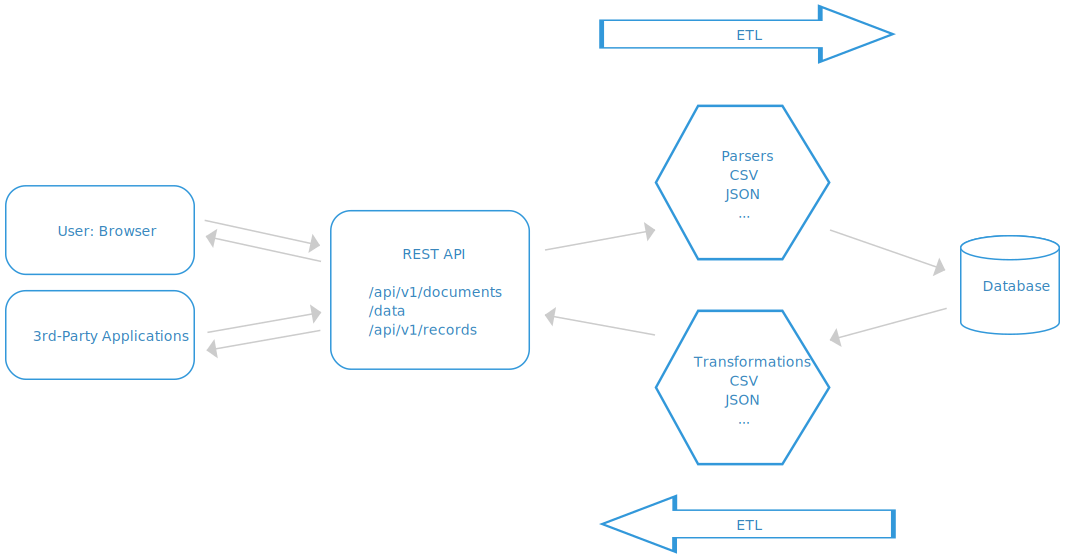
\includegraphics[width=\linewidth]{fig/ODH-Architecture-Overview}
    \caption{Grobe Architektur-Übersicht}
    \label{fig:pd:arch-overview}
\end{figure}

\subsection{Komponenten}


\subsection{Klassen}


\subsection{Sequenzdiagramm}



\section{User Interface}
\subsection{Authentifizierung}
Zur Authentifizierung der Benutzer wird der oAuth 2 Standard verwendet. Dieser erlaubt ein Login mit einem GitHub, FaceBook oder anderem Konto. Implementiert wurde dieser Standart auf der REST Seite mit hilfe von verschiedenen Django Plugins. 
Beispielsweise wurde python-social-auth verwendet um den Benutzer gegenüber diesen Diensten zu authentisieren. Die REST Schnittstelle wird dann über einen Token gesichtert.


\section{Testing}


\chapter{Resultate und Ausblick}

\section{Resultate}


\section{Weiterentwicklung}


